\subsection{Barycentric coordinates}\label{section:barycentric-coord}
Barycentric coordinates, discovered by M\"obius in 1827, consist of one of the most progessive area of research in computer graphics and mathematics thanks to the numerous applications in image and geometry processing.
\cite{REPORT:localbarycentricoordsepfl}
% ------
The position of any point in a triangle can be expressed using a linear combination with three scalars using barycentric coordinates:
$$ p = \lambda_1 p_1 + \lambda_2 p_2 + \lambda_3 p_3$$
where $p_1$, $p_2$ and $p_3$ are the vertices of a triangle and $\lambda_1$, $\lambda_2$ and $\lambda_3$ (the barycentric coordinates) are three scalars such that
respect the following barycentric coordinates properties.\cite{SLIDE:ICORSI}
% -------
\begin{itemize}
  \item partition of unity: $\sum_{i=1}^3 \lambda_{i}(p) = 1$
  \item reproduction: $\sum_{i=1}^3 \lambda_{i}(p)p_i = p$
  \item Lagrange-property: $\lambda_i(p_j) = \delta_{i, j}$
  \item linearity: $\lambda_i \in \prod_1$
  \item non-negativity: $\lambda_i(p)\geq 0$ for $p \in [p_1, p_2, p_3]$
\end{itemize}

% -------
A point is inside the triangle if and only if $0 \leq \lambda_1, \lambda_2, \lambda_3 \leq 1$. If a barycentric coordinates is less than zero or greater than one, the point is outside the triangle.
% -------
Barycentric coordinates allow the interpolation of values from a set of control points over the interior of a domain, using weighted combinations of values associated with the control points (Fig. \ref{fig:barycentric-coord}).
\cite{REPORT:localbarycentricoordsepfl}
% ------
\begin{figure}
  \centering
  \scalebox{.7}{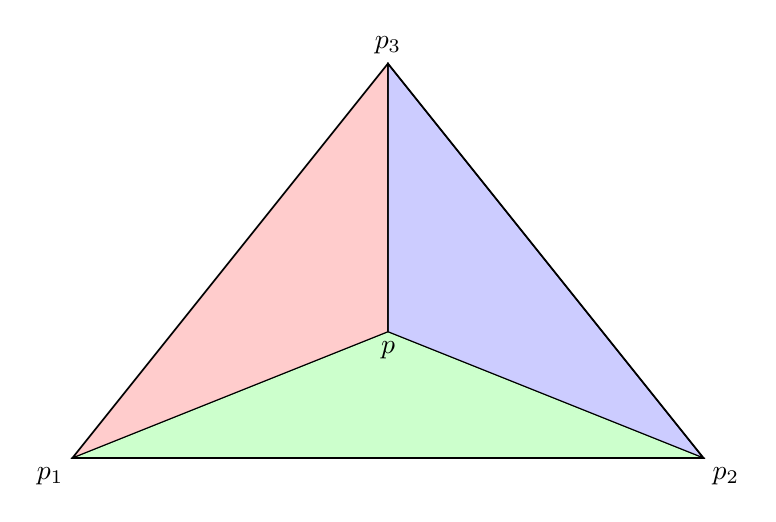
\begin{tikzpicture}
    \coordinate (L1) at (0,0);
    \coordinate (L2) at (8,0);
    \coordinate (L3) at (4,5);
    \coordinate (X) at (4,1.6);

    \draw[thick] (L1) -- coordinate[midway](md3) (L2)
                      -- coordinate[midway](md1) (L3)
                      -- coordinate[midway](md2) (L1) -- cycle;
    \filldraw[draw=black, fill=green!20] (L1) -- (X) -- (L2) -- cycle;
    \filldraw[draw=black, fill=red!20] (L1) -- (X) -- (L3) -- cycle;
    \filldraw[draw=black, fill=blue!20] (L3) -- (X) -- (L2) -- cycle;
    \draw (L1) node [below left] {$p_1$}
       -- (L2) node [below right] {$p_2$}
       -- (L3) node [above] {$p_3$}
       -- (X) node [below] {$p$};
    \end{tikzpicture}}
    \caption{Let $w_1$ be the blue area, $w_2$ the red one and $w_3$ the green one. Normalizing each of them by the area of the triangle, we will get three values ($\lambda_1, \lambda_2, \lambda_3$) that are the barycentric coordinates of $p$ with respect to the triangle [$p_1, p_2, p_3$].}
    \label{fig:barycentric-coord}
  \end{figure}

%%%%%%%%%%%%%%%%%%%%%%%%%%%%%%%%%%%%%%%%%%%%%%%%%%%%%%%%%%%%%%%%%

\subsection{Triangle meshes}
A collection of triangles without any particular mathematical structure is called \textit{triangle meshes}. To derive a global parameterization for an entire triangle mesh we can define a 2D position for each vertex. Let be $\mathcal{M}$ a triangle mesh that consists of a geometric and topological component represented by a graph structure with a set of vertices $\mathcal{V} = \{ v_1, ..., v_V \}$ and a set of triangular faces connecting them $\mathcal{F} = \{ f_1, ... , f_F \}$ with $f_i \in \mathcal{V} \times \mathcal{V} \times \mathcal{V}$. The connectivity of a triangle mesh can be expressed in termes of the edges of the respective graph $\mathcal{E} = \{ e_1, ..., e_E \}$ where $e_i \in \mathcal{V} \times \mathcal{V}$.
\cite{polygonmeshprocessing}
\begin{figure}[h!]
  \centering
  \minipage[b]{.5\linewidth}
  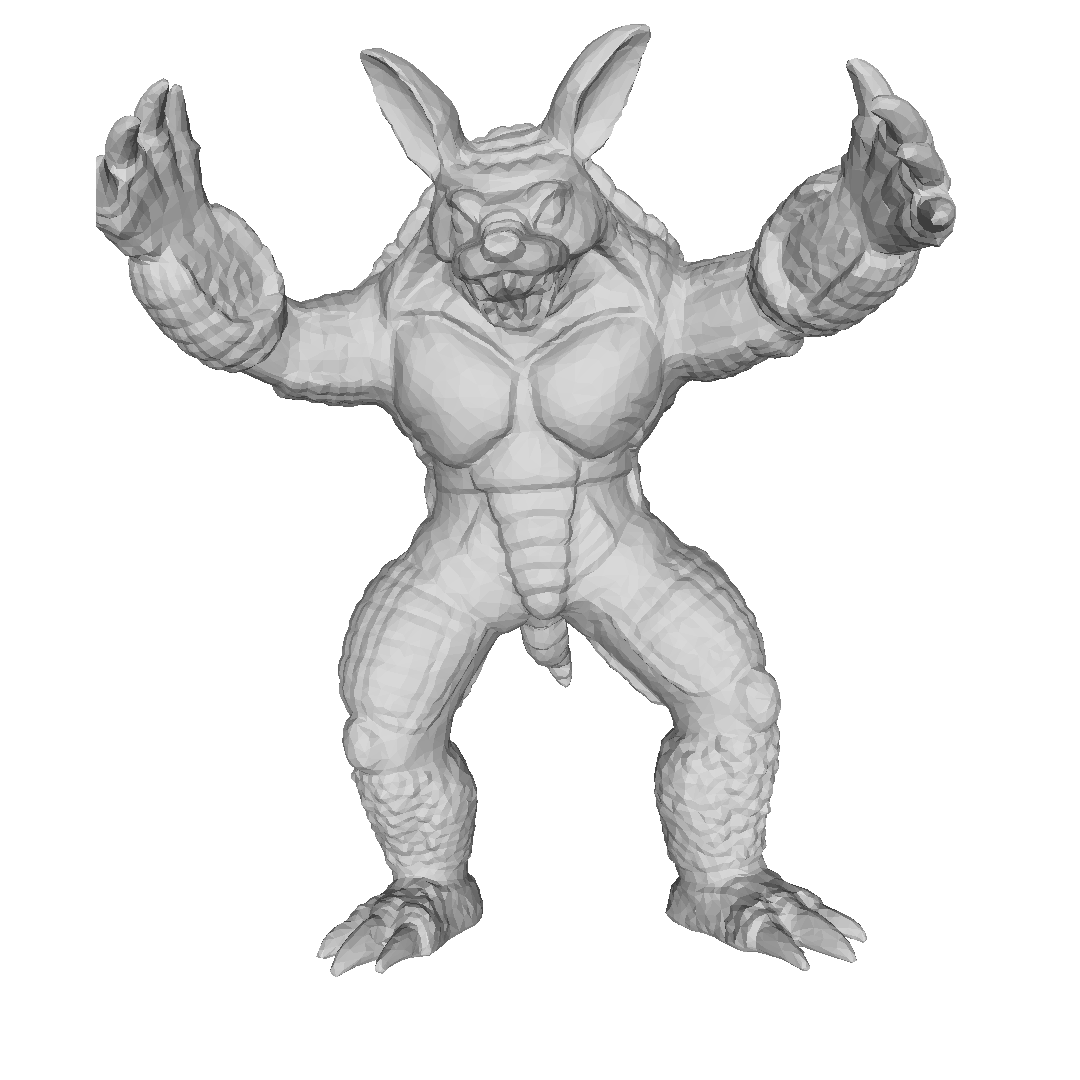
\includegraphics[scale=0.2]{images/armadillo-white04}
  \endminipage
  \minipage[b]{.5\linewidth}
  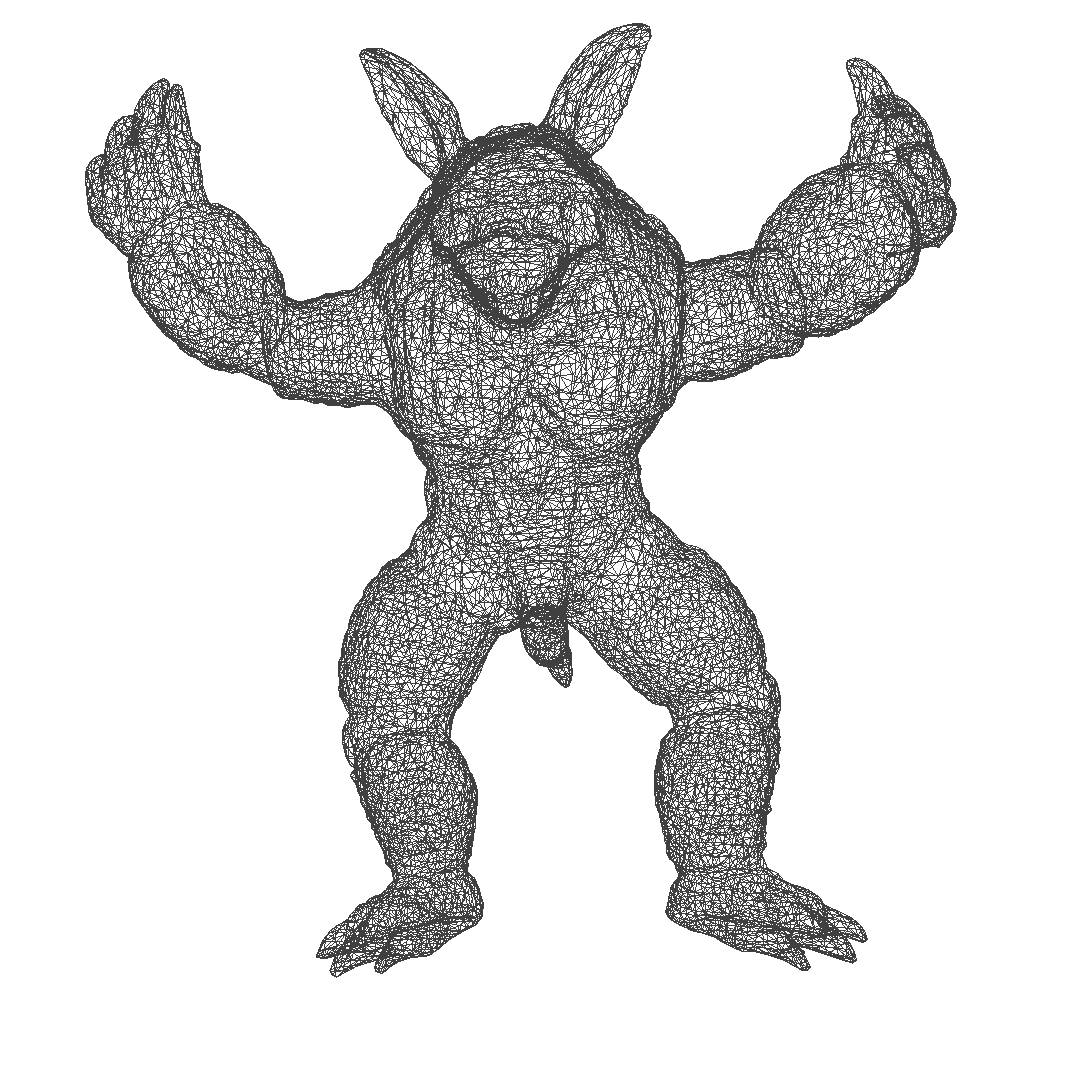
\includegraphics[scale=0.2]{images/armadillo-white205}
  \endminipage
\caption{3D triangle meshes.}

\end{figure}

%%%%%%%%%%%%%%%%%%%%%%%%%%%%%%%%%%%%%%%%%%%%%%%%%%%%%%%%%%%%%%%%%

\subsection{Lighting - Phong lighting model}

\begin{figure}[h!]
  \centering
  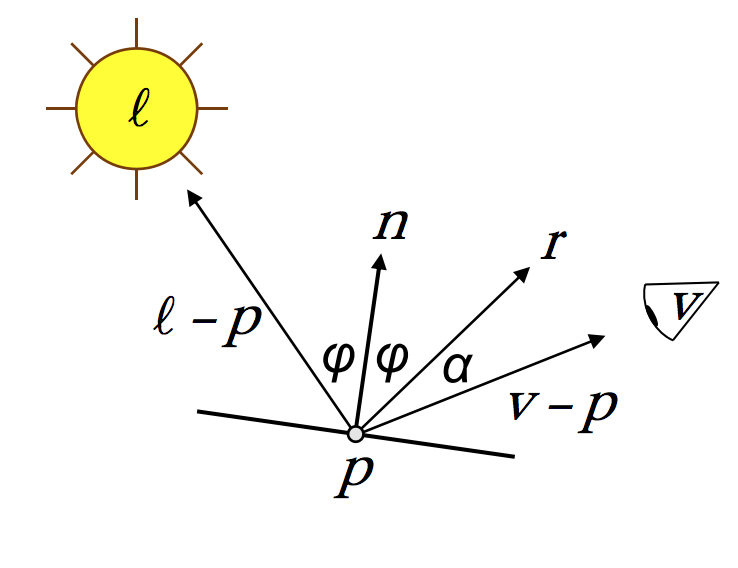
\includegraphics[scale=0.6]{images/lighting}
\caption{Lighting \cite{SLIDE:ICORSI}}
\end{figure}
Given a light source at position $l$ with intensity $I_l$ and a surface point at position $p$ with normal $n$,
we can define the angle between the incident light ($l-p$) and the normal $n$ as $\varphi$.
Let be $r$ our reflected light vector defined as $r = 2 n \cdot <n, l - p> - (l-p)$ and $\alpha$ the angle between that vector and the view direction $(v - p)$.

The \textit{Phong lighting model} is defined as the sum of the self-emitting intensity, ambient term, diffuse reflection and specular reflection.
$$ I = I_e + {\rho}_a \cdot I_A + \sum_{j=1}^n ({\rho}_d \cdot cos {\varphi}_j + {\rho}_s \cdot cos_{\alpha_j}^k) \cdot I_j$$ where $I_e$ is the self-emitting intensity, ${\rho}_a, {\rho}_d, {\rho}_s$ are the reflection constants (surface properties), $n$ is the number of lights sources with intensities $I_j$ and $k$ is the shininess.
\cite{SLIDE:ICORSI}

%%%%%%%%%%%%%%%%%%%%%%%%%%%%%%%%%%%%%%%%%%%%%%%%%%%%%%%%%%%%%%%%%

\subsection{Linear interpolation}\label{section:linear-interpolation}
Linear interpolation is an interpolation method where the result will return an equal spacing between the interpolated values. Given two numbers $n_1$ and $n_2$ (the start and final values of the interpolant), a linear interpolation can be made using a parameter $t$ ($t \in [0,1]$). \cite{WEBSITE:interpolation}

$$ n = n_1 + t (n_2 - n_1)$$


The standard linear interpolated visualisation is made passing three attributes (colours) to each vertex of a triangle. OpenGL will interpolate linearly these colors thanks to the barycentric coordinates that will tell how much of each color is being mixed at any position.
Given a triangle $[p_1, p_2, p_3]$, where the color blue is passed to vertex $p_1$, red to $p_2$, and green to $p_3$, let be $w_1$ the blue area, $w_2$ the red area and $w_3$ the green area (See Fig. \ref{fig:barycentric-coord}). Let define the value at $p$ as a \textit{barycentric interpolation} $$(w_1p_1 + w_2p_2 + w_3p_3)/W$$ where $W$ is the area of the triangle $[p_1, p_2, p_3]$.

%%%%%%%%%%%%%%%%%%%%%%%%%%%%%%%%%%%%%%%%%%%%%%%%%%%%%%%%%%%%%%%%%

\subsection{Flat Shading}
\textit{Flat shading} is a way to compute the colour at each pixel (at a corner or the barycentre) using the triangle normal.
Given a triangle $[p_1, p_2, p_3]$, the lighting is computed using the normal $n$ $$\widehat{n} = (p_2 - p_1) \times (p_3 - p_1) \;\;\;\;\;\;\;\; n = \frac{ \widehat{n} } { ||\widehat{n}|| } $$ at $p= (p_1 + p_2 + p_3)/3$. This colour is then used for all pixels. Flat shading gives objects with flat facets.
\cite{SLIDE:ICORSI}
%%%%%%%%%%%%%%%%%%%%%%%%%%%%%%%%%%%%%%%%%%%%%%%%%%%%%%%%%%%%%%%%%

\subsection{Gouraud Shading}
\textit{Gouraud Shading} is a way to compute the colour at each pixel assigning a normal to each corner and after having computed the color for each corner it linearly interpolates these colour values (see Sections \ref{section:barycentric-coord} and \ref{section:linear-interpolation}).
Given a triangle $[p_1, p_2, p_3]$ and the normal at each corner $n_1, n_2, n_3$.
The lighting is computed at $p_i$ using normal $n_i$ this applied to each corner return the colour values $c_1, c_2, c_3$.
These colors are then linearly interpolate $c = {\mu}_1 c_1 + {\mu}_2 c_2 + {\mu}_3 c_3$. Gouraud shading gives objects that appear more curved. \cite{SLIDE:ICORSI}

%%%%%%%%%%%%%%%%%%%%%%%%%%%%%%%%%%%%%%%%%%%%%%%%%%%%%%%%%%%%%%%%%

\subsection{Local averaging regions} \label{section:localaveraging}
A mesh can be constructed either as the limit of a family of smooth surfaces or as a linear approximation of an arbitrary surface. To derive a spatial average of geometric properties we mix finite elements (a linear interpolation between three vertices of a triangle) and finite volumes (finite-volume region on a triangulated surface using Voronoi cells or Barycentric cells, Fig. \ref{fig:localregions}). Restricting the average to the neighboring triangles (\textit{1-ring}) we can choose for each vertex an associated surface patch over which the average will be computed.
Let $\mathcal{A}_{Barycenter}$ be the area formed using barycenters and $\mathcal{A}_{Voronoi}$ the one formed using \textit{Voronoi} cell. The general case is represented by a point that can be anywhere, let's denote this surface area $\mathcal{A}_M$.

\begin{figure}[!h]
    \centering
    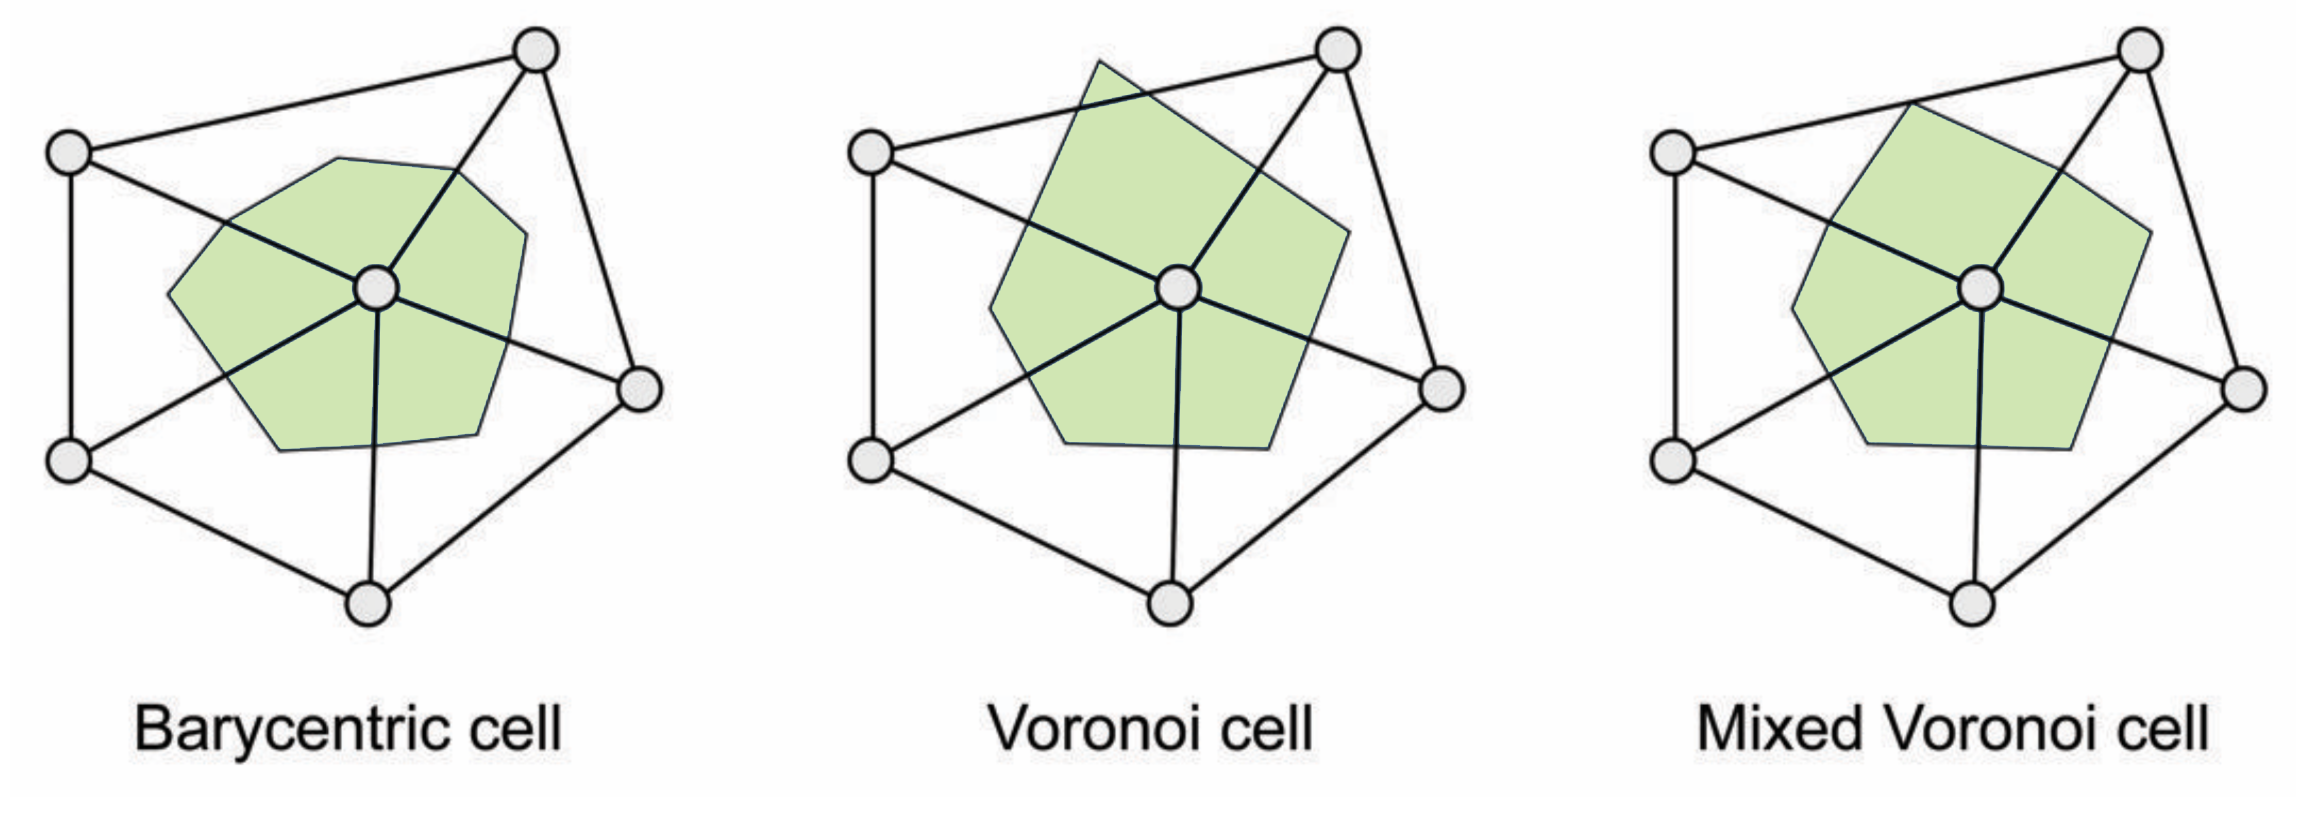
\includegraphics[scale=0.35]{images/localregions.png}
    \label{fig:localregions}
    \caption{Local averaging regions used for computing discrete differential operators associated with the center vertex of the one-ring neighborhood.\cite{polygonmeshprocessing}}
\end{figure}
\textit{Voronoi} cell of each vertex is an appropriate local region that provide a stable error bounds.
The \textit{Voronoi} region for a point $P$ of a triangle non-obtuse $[P, Q, R]$ is expressed as $\frac{1}{8}(| PR|^2 cot \angle Q + |PQ |^2 cot \angle R)$. The sum of these areas for the whole \textit{1-ring neighborhood} gives the non-obtuse \textit{Voronoi} area for a vertex. The above expression for the \textit{Voronoi} finite-volume area does not hold in case of obtuse angles. Let's define a new surface area for each vertex denoted $\mathcal{A}_{Mixed}$. Essentially the idea is to use the circumcenter point for each non-obtuse triangle and to use the midpoint of the edge opposite to the obtuse angle in case of an obtuse triangle. (See Pseudocode \ref{appendix:localaveraging}).\cite{meshlab}

\subsection{Gaussian Curvature} \label{section:gaussian-curvature-intro}
The \textit{Gaussian curvature} $K$ is defined as the product of the principal curvatures (square of the geometric mean):
$$K=k_1k_2$$
where $k_1$ and $k_2$ are the principal directions. A basic interpretation should be to imagine the \textit{Gaussian curvature} like a logical \texttt{AND} since it will check if there is a curvature along both directions.
The curvature of a surface is characterized by the principal curvatures, the \textit{Gaussian curvature} and the \textit{mean curvature} are simply averages of them.
\cite{WEBSITE:gaussiancurvaturedirty}
%---------
\begin{figure}[h]
  \centering
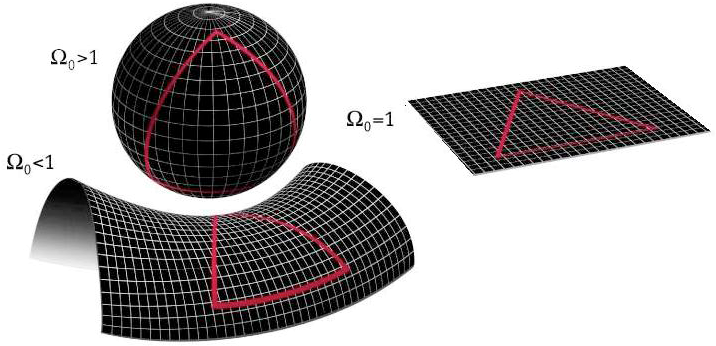
\includegraphics[scale=0.5]{images/gaussian_curvature_examples.png}
\caption{Positive curvature, negative curvature and zero curvature.}\label{fig:curvature-gaussian}
\end{figure}
Surfaces that have a zero gaussian curvature are called \textit{developable surfaces} because they can be flattened out into the plane without any stretching. \textit{Gaussian curvature} should be zero inside each mesh triangle and the same along edges since it can be flattened symmetrically into the plane by simply rotating one triangle about the common edge into the plane defined by the other. Consequently the \textit{Gaussian curvature} is concentrated at the vertices of a triangle and defined as the \textit{angle defect}
$$K(V) = 2 \pi - \sum_{i=1}^n \theta_i$$
where $\theta_i$ are the angles of the triangle $T_i$ adjacent to the vertex $V$ at $V$. This should be seen as the integral of the Gaussian curvature over a certain region $S(V)$ around $V$, where these $S(V)$ form a partition of the surface of the entire mesh.
$$ K(V) = \int_{S(V)} KdA  $$
\textit{Negative curvature} can be recognized by the fact that external directions curve in opposite directions, \textit{zero curvature} has one external direction that has zero curvature, \textit{positive curvature} has external directions that curve in the same direction (Fig. \ref{fig:curvature-gaussian}).
The \textit{Theorema Egregium}, discovered by C.F. Gauss in 1827, states that the \textit{Gaussian curvature} is an intrinsic property of the surface that does not depend on the space, despite by the fact that is define as the product of the principal curvatures (whose value depends on how the surface is immersed in the space). Technically, the \textit{Gaussian curvature} is invariant under isometries.
We can then notice that triangle angles add up to less than $180 \degree$ in negative curature, exactly $180 \degree$ in zero curature, and more than $180 \degree$ in positive curature.
\cite{geometryprocessing}
%%%%%%%%%%%%%%%%%%%%%%%%%%%%%%%%%%%%%%%%%%%%%%%%%%%%%%%%%%%%%%%%%

\subsection{Mean Curvature}
The \textit{mean curvature} H is defined as the arithmetic mean of principal curvatures : $$H = \frac{k_1 + k_2}{2}$$ where $k_1$ and $k_2$ are the principal directions. A basic interpretation should be to imagine the \textit{mean curvature} like a logical \texttt{OR} since it will check if there is a curvature along at least one direction.\cite{WEBSITE:gaussiancurvaturedirty}
The \textit{mean curvature} inside each mesh triangle is zero, but it does not vanish at edges. The \textit{mean curvature} associated with an edge is defined as $H(E) = \parallel E \parallel {\theta}_E/2$ where ${\theta}_E/2$ is the signed
angle between the normals of adjacent triangles (see Fig. \ref{fig:mean-curvature}).

\begin{figure}[h]
  \centering
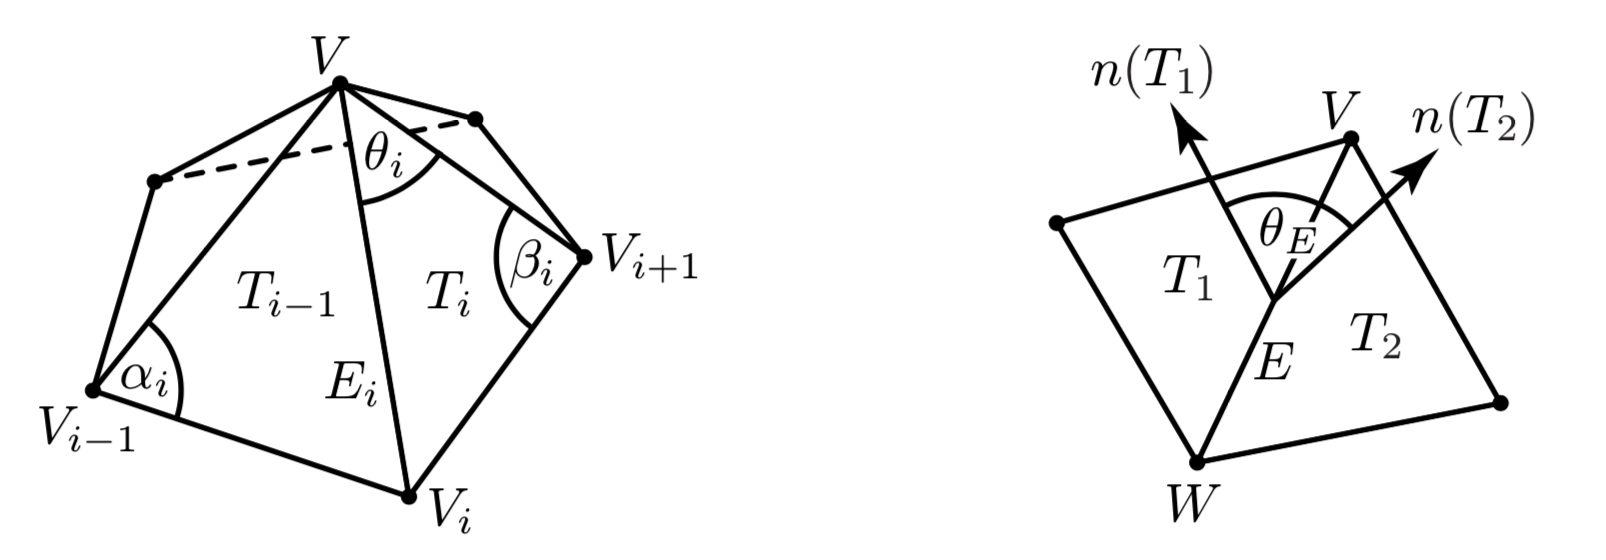
\includegraphics[scale=0.4]{images/mean_curvature_paper.png}
\caption{A vertex $V$ with its neighbouring vertices $V_i$ and adjacent triangles $T_i$. Angles opposite the edge $E_i$ are denoted by $\alpha_i$ and $\beta_i$. The
angle between the normals of adjacent triangles $T_1$ and $T_2$ with positive or negative sign is denoted as ${\theta}_E$.\cite{geometryprocessing}}\label{fig:mean-curvature}
\end{figure}
Let's think of an edge as a cylindrical patch $C(E)$ with a radius $r$ that touches the planes defined by adjacent triangles. The \textit{mean curvature} at any point of the cylindrical patch is defined as $1/(2r)$ and the area of $C(E)$ is $r||E||\theta_E$
$$H(E) = \int_{C(E)} HdA$$
//TODO: finish!!!!!!!!!!!!!!!!!
The \textit{mean curvature} at a vertex $V$ is defined as:
$$ H(V) = \frac{1}{2} \sum_{i=1}^n H(E_i)$$ Averaging the mean curvatures of its adjacent edges guarantee that \textit{mean curvature} of an edge is divide uniformly to both end points.
\cite{geometryprocessing}


